% B.Tech. Project I -- Mid-Semester Report
% Build: pdflatex main.tex (twice, for the table of contents and references), or upload
% the whole report/ folder to Overleaf. Figures are in figures/; diagrams are drawn with TikZ.
\documentclass[11pt,a4paper]{article}

\usepackage[margin=2.3cm]{geometry}
\usepackage[T1]{fontenc}
\usepackage{lmodern}
\usepackage{microtype}
\usepackage{graphicx}
\usepackage{amsmath,amssymb}
\usepackage{booktabs,tabularx,array,multirow}
\usepackage{xcolor}
\usepackage{enumitem}
\usepackage{caption}
\usepackage{float}
\usepackage{tikz}
\usetikzlibrary{arrows.meta,positioning,calc,fit,shapes.misc,shapes.geometric}
\usepackage[hidelinks]{hyperref}

\setlist{itemsep=2pt,topsep=4pt}
\captionsetup{font=small,labelfont=bf}
\renewcommand{\arraystretch}{1.15}
\newcolumntype{L}{>{\raggedright\arraybackslash}X}

% ---------------------------------------------------------------- front-page details
\newcommand{\projecttitle}{Topology-Aware Graph Representation for Deep Reinforcement Learning-Based Routing on MEDA Biochips}
\newcommand{\supervisorname}{Dr Ankur Gupta}
\newcommand{\supervisordept}{Dept. of Computer Science and Engineering}

% TikZ styles
\tikzset{
  blk/.style={draw, rounded corners=2pt, align=center, font=\small, minimum height=8mm, inner sep=4pt, fill=#1},
  blk/.default=white,
  arr/.style={-{Stealth[length=2.2mm]}, thick},
}
\definecolor{base}{HTML}{FBE3E3}
\definecolor{prop}{HTML}{DDEBFA}
\definecolor{same}{HTML}{EDEDED}
\definecolor{done}{HTML}{DFF1DF}
\definecolor{todo}{HTML}{FFF2CC}

\begin{document}
\pagenumbering{Alph}
% ================================================================= FRONT PAGE
\begin{titlepage}
  \centering
  {\Large\bfseries B.Tech Project -- I: 7th Semester\par}
  {\large Mid-Semester Report\par}
  \vspace{1.2cm}
  \IfFileExists{figures/nsut_logo.png}{
\includegraphics[width=0.42\textwidth]{figures/nsut_logo.png}}%
    {\fbox{\parbox[c][5cm][c]{5cm}{\centering NSUT logo\\(figures/nsut\_logo.png)}}}\par
  \vspace{1.2cm}
  {\LARGE\bfseries \projecttitle\par}
  \vspace{1.6cm}
  \begin{flushleft}
  \hspace*{2.2cm}\begin{minipage}{0.8\textwidth}
    \textbf{By:}\\[2pt]
    Aman Bihari (2023UCA1910)\\
    Deepak (2023UCA1913)\\
    Deepak (2023UCA1914)\\[1.2cm]
    \textbf{Supervisor:}\\[1.4cm]
    \supervisorname\\
    (\supervisordept)
  \end{minipage}
  \end{flushleft}
  \vfill
  {\large Netaji Subhas University of Technology, New Delhi\\ September 2026\par}
\end{titlepage}
\pagenumbering{roman}
% ================================================================= TABLE OF CONTENTS
\begin{center}
{\Large\bfseries Table of Contents}\\[0.6cm]
\begin{tabular}{|p{1.2cm}|p{9.6cm}|p{1.3cm}|p{2.2cm}|}
\hline
\textbf{S.No} & \textbf{Section} & \textbf{Page} & \textbf{Sign.} \\ \hline
1)  & Abstract                               & \pageref{sec:abstract}   & \\[10pt] \hline
2)  & Introduction                           & \pageref{sec:intro}      & \\[10pt] \hline
3)  & Motivation                             & \pageref{sec:motivation} & \\[10pt] \hline
4)  & Literature Survey                      & \pageref{sec:lit}        & \\[10pt] \hline
5)  & Problem Statement                      & \pageref{sec:problem}    & \\[10pt] \hline
6)  & Objectives and Methodology             & \pageref{sec:method}     & \\[10pt] \hline
7)  & Simulation Platform and Requirements   & \pageref{sec:platform}   & \\[10pt] \hline
8)  & Preliminary Results                    & \pageref{sec:results}    & \\[10pt] \hline
9)  & Conclusion and Future Work             & \pageref{sec:conclusion} & \\[10pt] \hline
10) & References                             & \pageref{sec:refs}       & \\[10pt] \hline
\end{tabular}
\end{center}
\thispagestyle{empty}
\newpage
\pagenumbering{arabic}

% ================================================================= ABSTRACT
\section*{Abstract}\label{sec:abstract}
Micro-electrode-dot-array (MEDA) biochips transport nanolitre droplets over a
grid of micro-electrode cells (MCs) whose electrodes degrade with use, so that
droplet movement becomes stochastic. Elfar et al.\ \cite{elfar2023} address
reliable routing with deep reinforcement learning: a convolutional neural
network (CNN) encodes the sensed MC health together with the droplet and goal
locations as a three-channel image, and Proximal Policy Optimization (PPO)
learns the routing policy. Taking this CNN--PPO method as the baseline, this
work investigates a topology-aware alternative in which each MC is a graph
node connected to its eight neighbours, a Graph Convolutional Network (GCN) encodes
the graph, and global max pooling provides the state
representation for the same PPO learner.
In single-seed experiments on healthy chips, the GCN with isotropic message
passing did not learn to route (4.0\% and 2.8\% success on held-out jobs on
$16\times16$ and $30\times30$ chips): its graph embedding is invariant to the
mirror and rotation symmetries of the chip, so the policy cannot distinguish a
job from its mirror images and rotations, although these require different
directions. A direction-aware GCN, with a separate
weight matrix for each neighbour direction, removes this limitation; it is
equivalent to a three-layer convolutional network with global max pooling and
has 76\,k encoder parameters, against 29.7\,M for the baseline CNN. After 40
training epochs on $30\times30$ chips it routed all 500 held-out jobs in 9.84
cycles on average, against 87.4\% success and 14.52 cycles for the CNN--PPO
baseline, which had not converged. On chips of up to $100\times100$ MCs its
success rate remained at or above 99.6\%, while that of the baseline fell to
15.6\% (the baseline converged at no size); on $120\times120$ chips, where a time limit stopped its training after
21 of 40 epochs, it reached 89.2\% against 10.2\%. A comparison with the
authors' original implementation (three seeds each) gave no indication that our
implementation of the baseline learns more slowly than the original.

% ================================================================= 1. INTRODUCTION
\section{Introduction}\label{sec:intro}

\paragraph{Digital microfluidics and MEDA biochips:}
Digital microfluidic biochips automate biochemical protocols by manipulating
discrete droplets on a planar array of electrodes using
electrowetting-on-dielectric (EWOD) \cite{pollack2000,chakrabarty2006}.
The micro-electrode-dot-array (MEDA) architecture refines this concept: the
chip consists of thousands of identical micro-electrode cells (MCs), each with
its own control and sensing circuitry \cite{wang2011,li2017}. A droplet covers
a rectangle of several MCs and is moved by actuating the MCs adjacent to its
leading edge. Because each MC also senses its own state, the controller has
real-time information about the chip.

\paragraph{Droplet routing:}
A bioassay is executed as a sequence of fluidic operations (dispensing, mixing,
splitting and detection), between which droplets are transported across the
chip. Each routing job moves a droplet of a given size from a start location
to a goal location within a permitted routing zone. At every control cycle,
the routing policy selects the direction in which the droplet is moved.

\paragraph{Reliability and MC degradation:}
Repeated actuation causes charge trapping in the dielectric, so that the EWOD
force of an MC decreases with its number of actuations. A droplet whose
leading edge lies over degraded MCs may move more slowly than commanded or not
at all \cite{elfar2023}. Routing therefore cannot follow the geometrically
shortest path alone; it must account for the current health of the MCs and
adapt as the chip ages.

\paragraph{Reinforcement learning and the base paper:}
Elfar et al.\ \cite{elfar2022date,elfar2023} formulate adaptive routing as a
sequential decision problem and solve it with deep reinforcement learning.
The agent observes a three-channel grid (MC health, droplet location and goal
location), which a CNN encodes; a PPO actor--critic \cite{schulman2017}
selects one of eight movement directions. In this architecture the CNN serves
as the state encoder and PPO as the learning algorithm, comprising an actor
(policy) and a critic (value function).

\paragraph{Scope of this work:}
This work takes the CNN--PPO method of Elfar et al.\ \cite{elfar2023} as the
baseline and investigates replacing only its state encoder with a GCN
operating on an explicit MC graph; the simulation environment, reward, action
space and PPO learner are identical for all compared configurations. On chips
larger than $30\times30$ MCs, the baseline observes the chip resampled to
$30\times30$, as in \cite{elfar2023}, whereas the GCN operates on the native MC
grid, so the observation resolution differs as well.

% ================================================================= 2 MOTIVATION
\section{Motivation}\label{sec:motivation}

A MEDA chip is physically a set of MCs with fixed spatial neighbourhoods, and
routing decisions depend on how health values, the droplet and the goal are
arranged within those neighbourhoods. This structure shows a direct graph
abstraction: each MC becomes a node, each pair of spatially adjacent MCs is
joined by an edge, and the per-MC observation values become node features.

A CNN captures local spatial relationships through its convolution kernels.
The baseline, however, treats the chip as an image of fixed size: every chip
is resampled to a $30\times30$ observation, and the fully connected layer
after the convolutions accounts for 29.5 of the 29.7 million parameters of the
Table~I network \cite{elfar2023}. A GCN applies the same weights at every
node; its parameter count is independent of the chip size, and it operates on
the native MC grid of any chip. This work investigates whether such an
explicit, topology-aware representation is an effective state encoder for
PPO-based routing.

The graph representation is read out with \emph{global max pooling}, the
element-wise maximum over all node embeddings. Its adequacy as a readout for
routing is evaluated experimentally.

% ================================================================= 3 LITERATURE SURVEY
\section{Literature Survey}\label{sec:lit}

\paragraph{Digital microfluidics and MEDA:}
EWOD-based droplet actuation was demonstrated by Pollack et al.\ \cite{pollack2000},
and design-automation methods for digital microfluidic biochips (synthesis,
testing and reconfiguration) are surveyed by Chakrabarty and Su
\cite{chakrabarty2006}. Wang et al.\ \cite{wang2011} introduced the MEDA
architecture, whose fine-grained MCs allow droplets of different sizes and
shapes. Li et al.\ \cite{li2017} developed droplet-size-aware synthesis that
exploits this flexibility.

\paragraph{Classical and formal droplet routing:}
Early work treated droplet routing as a combinatorial problem on a fixed
electrode grid. Su et al.\ \cite{su2006} routed droplets as part of biochip
synthesis while avoiding droplet interference. These methods assume that
electrodes behave ideally. Elfar et al.\ \cite{elfar2021date,elfar2022tcad}
modelled MC degradation and stochastic droplet movement explicitly and
synthesized routing strategies with formal methods (stochastic games solved
with PRISM-games), which are reliable but become costly as chips and bioassays
grow.

\paragraph{Reinforcement learning for routing:}
Liang et al.\ \cite{liang2020} applied deep reinforcement learning to
adaptive droplet routing on conventional digital microfluidic biochips and
later extended it to parallel control of multiple droplets on MEDA with
multi-agent reinforcement learning \cite{liang2021}. Elfar et al.\
\cite{elfar2022date,elfar2023} route droplets on MEDA biochips with a CNN--PPO
agent that observes the sensed MC health, using a parameterized action space
whose step size adapts to the droplet size, and transfer learning across chip
sizes. Their evaluation includes COVID-19 bioassays and experiments on
fabricated prototypes.

\paragraph{Graph neural networks and graph-based reinforcement learning:}
Message-passing neural networks \cite{gilmer2017} update each node's
embedding from its neighbours. The Graph Convolutional Network (GCN)
\cite{kipf2017} does so with a normalized neighbourhood average, and
GraphSAGE \cite{hamilton2017} generalizes aggregation to unseen graphs.
Relational GCNs \cite{schlichtkrull2018} learn separate weights per edge
type. Xu et al.\ \cite{xu2019} analyse how the aggregation and readout
functions bound the discriminative power of message-passing graph networks,
which is relevant to the choice of global max pooling. Beaini et al.\
\cite{beaini2021} argued that the
isotropic aggregation of most graph networks cannot capture directions and
proposed directional aggregation, a limitation that this work encounters on
the MC grid. Graph encoders have also been combined with reinforcement
learning: Zambaldi et al.\ \cite{zambaldi2019} introduced relational inductive
biases into deep reinforcement learning agents, Jiang et al.\ \cite{jiang2021}
represented grid observations as graphs whose edge types encode spatial
relations, and in macro placement for chip design an edge-based graph network
encodes the netlist for a policy trained with PPO \cite{mirhoseini2021}.

\paragraph{Position of this work:}
The surveyed MEDA routing methods encode the chip state either as formal
models \cite{elfar2022tcad} or as images for a CNN \cite{elfar2023,liang2021}.
None represents the MC array as a graph for a GCN encoder. This work studies
that representation while keeping the simulation environment, reward, action
space and PPO learner identical across all compared configurations, so that
differences in performance can be attributed to the state encoder, together
with the observation resolution on chips larger than $30\times30$ MCs.

% ================================================================= 4 PROBLEM STATEMENT
\section{Problem Statement}\label{sec:problem}

\paragraph{Routing job and chip model:}
A $W\times H$ chip holds MCs indexed by $(x,y)$. A droplet is the rectangle
$\delta=(x_a,y_a,x_b,y_b)$ of MCs it covers. A routing job
$(\delta_s,\delta_g,\delta_h)$ requires the droplet to be moved from the start
$\delta_s$ to the goal $\delta_g$ within the routing (hazard) zone
$\delta_h$. Following the base paper \cite{elfar2023}, the degradation of MC
$(i,j)$ after $n_{ij}$ actuations and its sensed health are
\begin{equation}
  D_{ij}=\tau_{ij}^{\,n_{ij}/c_{ij}}, \qquad
  H_{ij}=\min\!\big(\big\lfloor 2^{b} D_{ij}\big\rfloor,\ 2^{b}-1\big),
\end{equation}
with $\tau_{ij}\in[0.5,0.7]$ and $c_{ij}\in[500,800]$ fitted from
measurements, and a $b$-bit health sensor. A move succeeds stochastically
with a probability determined by the degradation of the MCs at the droplet's
leading edge, and every actuation increases their $n_{ij}$.

\paragraph{Reinforcement-learning formulation (baseline):}
\begin{itemize}
  \item \textbf{State:} a three-channel $W\times H$ grid of MC health
        ($H/2^b$ inside the routing zone, 0 outside), droplet location and
        goal location.
  \item \textbf{Actions:} eight directions (N, S, E, W, NE, NW, SE, SW). The
        step size adapts to the droplet size and never overshoots the goal
        (Algorithm~1 of \cite{elfar2023}).
  \item \textbf{Transition:} the stochastic, health-dependent droplet movement
        of the simulator.
  \item \textbf{Reward:} $r = a_{dis}\,r_{dis} + a_{ter}\,r_{ter} + a_{act}\,r_{act}$,
        combining progress towards the goal, a terminal reward on arrival and a
        penalty for invalid actions \cite{elfar2023}; the implemented
        coefficients follow the reference code \cite{elfarcode}, which
        rewards progress and penalizes moves away from the goal asymmetrically
        (Table~\ref{tab:params}).
  \item \textbf{Termination:} the droplet reaches the goal, or $k_{\max}$
        control cycles elapse.
  \item \textbf{Learner:} PPO with an actor--critic network \cite{schulman2017}.
\end{itemize}

\paragraph{Representation problem:}
The baseline encodes the state as
\emph{3-channel grid $\rightarrow$ CNN $\rightarrow$ Flatten $\rightarrow$ PPO}.
This work studies the alternative
\emph{MC graph $\rightarrow$ GCN $\rightarrow$ global max pooling $\rightarrow$ PPO}
with the graph
\begin{equation}
  G=(V,E,X),\qquad N=|V|=WH,\qquad X\in\mathbb{R}^{N\times 3},
\end{equation}
where $V$ are the MC nodes, $E$ the spatial adjacencies and $X$ the three
baseline features per node. The problem is to determine whether this
representation enables PPO to learn reliable and efficient routing policies,
and how it compares with the CNN--PPO baseline under identical conditions.
Figure~\ref{fig:problem} shows a routing job in the simulator and the eight
movement actions.

\begin{figure}[H]
  \centering
  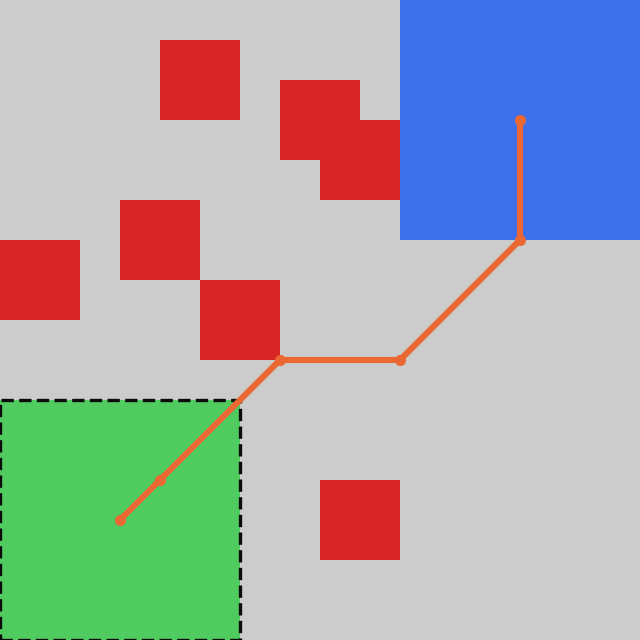
\includegraphics[width=0.36\textwidth]{figures/routing_example.png}\hspace{6mm}
  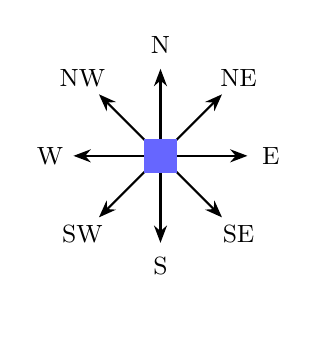
\begin{tikzpicture}[scale=0.85, baseline={(0,-2.2)}]
    \foreach \a/\l in {90/N,270/S,0/E,180/W,45/NE,135/NW,315/SE,225/SW}{
      \draw[arr] (0,0) -- (\a:1.3);
      \node[font=\small] at (\a:1.65) {\l};}
    \fill[blue!60] (-0.25,-0.25) rectangle (0.25,0.25);
  \end{tikzpicture}
  \caption{Left: a selected routing job on a $16\times16$ chip with 10\% faulty
    MCs in the simulator used in this work. The droplet (blue) is routed to the
    goal (green) around fully degraded MCs (red); the orange line is the path of
    the direction-aware GCN agent trained in this work on healthy chips.
    Right: the eight movement actions.}
  \label{fig:problem}
\end{figure}

% ================================================================= 5 OBJECTIVES AND METHODOLOGY
\section{Objectives and Methodology}\label{sec:method}

\begin{enumerate}[label=\textbf{O\arabic*.}]
  \item \textbf{Graph representation:} represent each MC as a node and
        spatially adjacent MCs as edges, retaining the state information of
        the baseline exactly.
  \item \textbf{GCN state encoding:} replace the CNN encoder with a GCN and a
        global max-pooling readout while retaining PPO.
  \item \textbf{Controlled evaluation:} compare the encoders under identical
        simulation, PPO settings, training budget (except where a time limit
        intervened) and held-out evaluation jobs.
\end{enumerate}

\subsection{Baseline (CNN--PPO)}
The baseline is the CNN--PPO method of Elfar et al.\ \cite{elfar2023}. Its
state encoder (Table~I in \cite{elfar2023}) has three convolutional layers
with 64, 128 and 128 filters, a 256-unit fully connected layer and eight
outputs; in the transfer-learning scheme of \cite{elfar2023}, every chip is
resampled to a $30\times30$ observation. Training uses 8 parallel environments
and $2^{14}$ environment steps per epoch, followed by an evaluation on 500
random routing jobs. The learning rate starts at $\eta_0=3.5\times10^{-4}$ and
is multiplied by $0.7$ whenever the evaluation success rate exceeds 99\%, with
a floor of $10^{-6}$. Details not specified in \cite{elfar2023} follow the
first author's public reference implementation \cite{elfarcode}: linear actor
(8 action logits) and critic ($V(s)$) heads share the encoder, and the reward
coefficients, the health-sensor resolution and the PPO hyperparameters are
taken from the same source, except where Table~\ref{tab:params} identifies a
value as assumed. The convolutions use $3\times3$ kernels with stride~1 and
zero padding, as in the reference implementation. In the preliminary $16\times16$ study, the baseline uses the
smaller CNN of the reference implementation (32, 64 and 64 filters and a
128-unit fully connected layer) at the native $16\times16$ resolution; the
$30\times30$ and chip-size studies use the Table~I network.

\subsection{Proposed methodology (GCN--PPO)}
Figure~\ref{fig:pipeline} shows the proposed pipeline. The baseline replaces
stages (b)--(d) with the CNN encoder; all other components are shared.

\begin{figure}[H]
\centering
\resizebox{\textwidth}{!}{%
\begin{tikzpicture}[>=Stealth, font=\small,
  lab/.style={align=center, font=\footnotesize, text width=2.9cm},
  flow/.style={->, thick}]
  % (a) observation
  \node[inner sep=0pt, draw=gray!60] (obs) at (0,0) {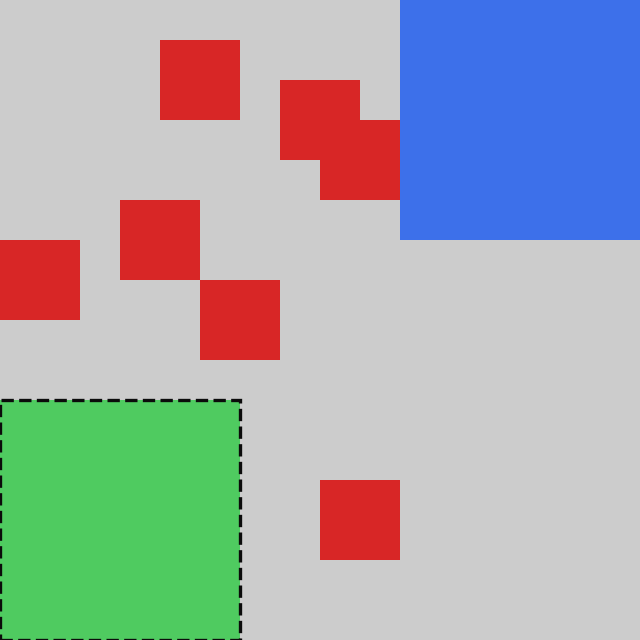
\includegraphics[width=2.3cm]{figures/routing_observation.png}};
  \node[lab, anchor=north] at (0,-1.45) {\textbf{(a) Observation}\\ health, droplet and goal channels};
  % (b) MC graph (4 x 3 excerpt)
  \begin{scope}[shift={(2.9,-0.7)}]
    \foreach \x in {0,...,3} \foreach \y in {0,...,2} {
      \ifnum\x<3 \draw[gray!60] (0.65*\x,0.7*\y) -- (0.65*\x+0.65,0.7*\y); \fi
      \ifnum\y<2 \draw[gray!60] (0.65*\x,0.7*\y) -- (0.65*\x,0.7*\y+0.7); \fi
      \ifnum\x<3 \ifnum\y<2
        \draw[gray!40] (0.65*\x,0.7*\y) -- (0.65*\x+0.65,0.7*\y+0.7);
        \draw[gray!40] (0.65*\x+0.65,0.7*\y) -- (0.65*\x,0.7*\y+0.7); \fi\fi }
    \foreach \x in {0,...,3} \foreach \y in {0,...,2}
      \node[circle, draw, fill=white, inner sep=0pt, minimum size=3.2mm] at (0.65*\x,0.7*\y) {};
    \foreach \p in {(0,0),(0.65,0)} \node[circle, draw, fill=blue!45, inner sep=0pt, minimum size=3.2mm] at \p {};
    \foreach \p in {(1.95,1.4),(1.3,1.4)} \node[circle, draw, fill=green!50!black!45, inner sep=0pt, minimum size=3.2mm] at \p {};
    \node[circle, draw, fill=red!55, inner sep=0pt, minimum size=3.2mm] at (1.3,0.7) {};
  \end{scope}
  \node[lab, anchor=north] at (3.875,-1.45) {\textbf{(b) MC graph}\\ $G=(V,E,X)$, 8-neighbour edges};
  % (c) three graph-convolution layers
  \foreach \i in {2,1,0}
    \draw[fill=prop, draw=blue!60!black, rounded corners=1.5pt] (6.3+0.2*\i,-0.95+0.2*\i) rectangle ++(1.7,1.5);
  \node[align=center, font=\footnotesize] at (7.15,-0.2) {GCN layer\\ $\times\,3$, $d=64$};
  \node[lab, anchor=north] at (7.35,-1.45) {\textbf{(c) Message passing}\\ $Z\in\mathbb{R}^{N\times 64}$};
  % (d) global max pooling: pooled vector
  \foreach \k/\s in {0/20,1/55,2/35,3/70,4/15,5/45,6/60,7/30}
    \draw[fill=blue!\s, draw=blue!60!black] (9.75,-0.95+0.24*\k) rectangle ++(0.34,0.24);
  \node[lab, anchor=north] at (9.92,-1.45) {\textbf{(d) Global max pooling}\\ $g\in\mathbb{R}^{64}$};
  % (e) PPO actor-critic
  \node[blk=same, minimum width=2.1cm] (actor) at (12.4,0.45) {Actor $\pi(a\,|\,s)$};
  \node[blk=same, minimum width=2.1cm] (critic) at (12.4,-0.55) {Critic $V(s)$};
  \node[lab, anchor=north] at (12.4,-1.45) {\textbf{(e) PPO}\\ actor--critic};
  % flow of the proposed pipeline
  \draw[flow] (1.25,0) -- (2.75,0);
  \draw[flow] (5.0,0) -- (6.2,0);
  \draw[flow] (8.5,0) -- (9.65,0);
  \draw[thick] (10.2,0) -- (10.6,0);
  \draw[flow] (10.6,0) -- (actor.west);
  \draw[flow] (10.6,0) -- (critic.west);
  \draw[flow] (actor.east) -- ++(1.1,0) node[right, font=\footnotesize, align=left] {action\\(1 of 8)};
  % baseline branch
  \node[blk=base, minimum width=5.6cm] (cnn) at (6.2,2.1) {Baseline encoder: CNN, 3 convolutional layers + FC};
  \draw[flow, dashed, red!60!black] (0,1.2) |- (cnn.west);
  \draw[thick, dashed, red!60!black] (cnn.east) -| (10.6,0);
\end{tikzpicture}}
\caption{GCN--PPO pipeline. (a) The simulator observation; (b) the MC graph
  with 8-neighbour edges (excerpt; droplet blue, goal green, degraded MC red);
  (c) three graph-convolution layers producing node embeddings; (d) global max
  pooling to a fixed-size graph embedding; (e) the PPO actor and critic. The
  dashed path is the CNN--PPO baseline, which replaces stages (b)--(d).}
\label{fig:pipeline}
\end{figure}

\paragraph{Graph construction:}
Each MC is one node, with the fixed index $\mathrm{node}(x,y)=y\,W+x$, which
is the row-major order of the observation tensor. Edges connect every MC to
its spatial neighbours in \textbf{eight directions} (left, right, up, down
and the four diagonals) and are stored in both directions. For a
$W\times H$ chip,
\begin{equation}
|E| = 2\big[(W-1)H + W(H-1) + 2(W-1)(H-1)\big],
\end{equation}
which gives 6\,844 directed edges on a $30\times30$ chip. Corner MCs have 3
neighbours, border MCs 5 and interior MCs 8. Edges encode adjacency only; the
health-dependent movement probabilities remain within the simulator, and a
degraded MC remains a node that carries its low health value
(Figure~\ref{fig:graph}).

\begin{figure}[H]
\centering
\resizebox{0.9\textwidth}{!}{%
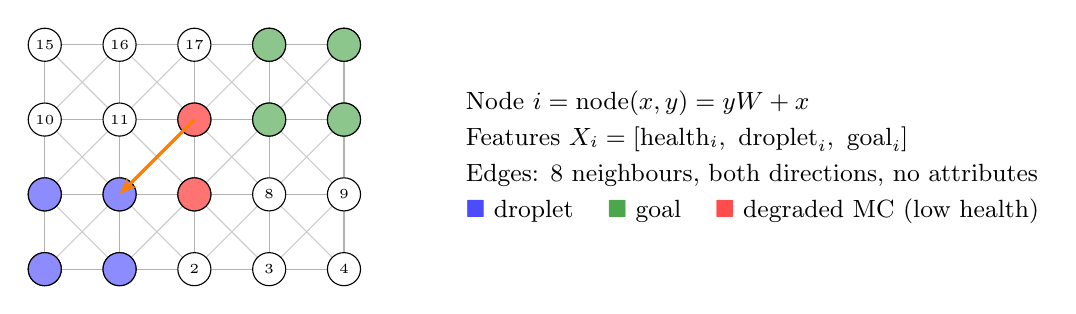
\begin{tikzpicture}[scale=0.95]
  \foreach \x in {0,...,4} \foreach \y in {0,...,3} {
    \ifnum\x<4 \draw[gray!60] (\x,\y) -- (\x+1,\y); \fi
    \ifnum\y<3 \draw[gray!60] (\x,\y) -- (\x,\y+1); \fi
    \ifnum\x<4 \ifnum\y<3 \draw[gray!40] (\x,\y) -- (\x+1,\y+1); \draw[gray!40] (\x+1,\y) -- (\x,\y+1); \fi\fi }
  \foreach \x in {0,...,4} \foreach \y in {0,...,3}
    \node[circle, draw, fill=white, inner sep=0pt, minimum size=4.2mm, font=\tiny] at (\x,\y) {\pgfmathparse{int(\y*5+\x)}\pgfmathresult};
  \foreach \p in {(0,0),(1,0),(0,1),(1,1)} \node[circle, draw, fill=blue!45, inner sep=0pt, minimum size=4.2mm] at \p {};
  \foreach \p in {(3,2),(4,2),(3,3),(4,3)} \node[circle, draw, fill=green!50!black!45, inner sep=0pt, minimum size=4.2mm] at \p {};
  \foreach \p in {(2,1),(2,2)} \node[circle, draw, fill=red!55, inner sep=0pt, minimum size=4.2mm] at \p {};
  \draw[arr, orange, very thick] (2,2) -- (1,1);
  \node[align=left, font=\small, anchor=west] at (5.5,1.5)
    {Node $i=\mathrm{node}(x,y)=yW+x$\\[2pt]
     Features $X_i=[\text{health}_i,\ \text{droplet}_i,\ \text{goal}_i]$\\[2pt]
     Edges: 8 neighbours, both directions, no attributes\\[2pt]
     \textcolor{blue!70}{$\blacksquare$} droplet \quad
     \textcolor{green!50!black!70}{$\blacksquare$} goal \quad
     \textcolor{red!70}{$\blacksquare$} degraded MC (low health)};
\end{tikzpicture}}
\caption{Graph construction on a $5\times4$ chip. Every MC is a node,
  numbered in row-major order and connected to up to eight neighbours. The
  orange arrow denotes one message, from a degraded MC to a droplet MC.}
\label{fig:graph}
\end{figure}

\paragraph{Node features:}
Node $i$ carries the three baseline values at its MC,
$X_i=[\text{health},\text{droplet},\text{goal}]$, copied from the observation
tensor without re-normalization. The implementation verifies this
correspondence element-wise, together with the node count, edge set, degrees
and batched tensor shapes.

\paragraph{Message passing:}
The encoder is a Graph Convolutional Network (GCN) \cite{kipf2017} with
$L=3$ layers, hidden dimension $d=64$ and ReLU activations:
\begin{equation}
  H^{(l+1)} = \mathrm{ReLU}\!\big(\hat{D}^{-1/2}\hat{A}\hat{D}^{-1/2} H^{(l)} W^{(l)} + b^{(l)}\big),
  \qquad \hat{A}=A+I,\quad H^{(0)}=X,
\end{equation}
producing node embeddings $Z=H^{(L)}\in\mathbb{R}^{N\times d}$. The number of layers and
the hidden dimension are design choices of this work (Table~\ref{tab:params}).

\paragraph{Direction-aware message passing:}
The direction-aware configuration replaces each GCN layer with a relational
graph convolution \cite{schlichtkrull2018} that has a separate weight matrix
for the node itself and for each of the eight neighbour directions $r$:
\begin{equation}
  h_i^{(l+1)} = \mathrm{ReLU}\Big(W_0^{(l)} h_i^{(l)} + \sum_{r=1}^{8}\sum_{j\in\mathcal{N}_r(i)} W_r^{(l)} h_j^{(l)} + b^{(l)}\Big),
\end{equation}
where $\mathcal{N}_r(i)$ contains the neighbour of MC $i$ in direction $r$,
if it exists. Edge directions are derived from the node indices, so the graph
carries no edge attributes, and messages are summed without degree
normalization. With $L=3$ and $d=64$, this encoder has 76\,k parameters.

\paragraph{Symmetry of isotropic message passing:}
Every mirror and rotation of a square chip (the eight elements of the dihedral
group $D_4$) maps the 8-neighbour grid onto itself, and the GCN weights each
neighbour independently of its direction; at MCs at least two cells from the
chip border, a GCN layer is a $3\times3$ convolution whose nine taps are
identical ($W/9$). The node embeddings of a
transformed job are therefore the correspondingly permuted node embeddings of
the original job, and any readout that ignores node order (maximum, mean or
sum) assigns both the same graph embedding. On a rectangular chip the same
holds for the two mirrors and the $180^\circ$ rotation. The policy, a linear
function of this embedding, cannot distinguish a job from its mirror images
and rotations. On a square chip, for a job whose goal lies straight along one axis from the
droplet, the eight transformed jobs require each of the four axis directions
twice; a policy with identical outputs for all eight chooses the direction of
the goal with probability at most $1/4$ on average over them.

\paragraph{Relation to convolution:}
Each direction-aware layer is a $3\times3$ convolution with stride~1 and zero
padding: $W_0^{(l)}$ is the centre tap, the weight $W_r^{(l)}$ of a neighbour
direction is the tap at that neighbour's position, and a neighbour missing at
the chip border contributes nothing, exactly as zero padding does. The
direction-aware GCN with global max pooling is therefore a three-layer fully
convolutional network followed by global max pooling, with
$1\,792+2\times36\,928=75\,648$ encoder parameters for any chip size. This
correspondence between relational graph convolutions over local directional
relations and $3\times3$ convolutions was noted by Jiang et al.\
\cite{jiang2021}; see also \cite{beaini2021}. Both
this equivalence and the symmetry of the isotropic GCN (for max, mean and sum
pooling) are verified numerically by automated tests. With $L=3$, each node
embedding depends only on the MCs within three hops, a $7\times7$ block of
MCs.

\paragraph{Global max pooling:}
The graph embedding is the element-wise maximum over all nodes,
\begin{equation}
  g_k=\max_{i\in V} Z_{i,k}, \qquad g\in\mathbb{R}^{d},
\end{equation}
which yields a fixed-size vector for any chip size.

\paragraph{Actor--critic:}
As in the baseline, linear heads on $g$ produce the actor's probabilities over
the eight actions and the critic's value estimate $V(s)$. The GCN encoder has
8.6\,k parameters, compared with 29.7\,M for the CNN of Table~I in
\cite{elfar2023}. Table~\ref{tab:compare} summarizes the differences between
the baseline and the proposed state encoder.

\begin{table}[H]
\centering\small
\begin{tabularx}{\textwidth}{lLL}
\toprule
Component & Baseline (CNN--PPO) & Proposed (GCN--PPO) \\ \midrule
State representation & 3-channel grid & MC graph $G=(V,E,X)$ \\
Encoder & CNN (Table~I of \cite{elfar2023}) & GCN, 3 layers, $d=64$ \\
Spatial structure & implicit, via $3\times3$ convolutions & explicit 8-neighbour edges \\
Features & health, droplet, goal & health, droplet, goal \\
Readout & flatten + FC 256 & global max pooling \\
\bottomrule
\end{tabularx}
\caption{Comparison of the baseline and the proposed state encoder.}
\label{tab:compare}
\end{table}

\subsection{Training and evaluation procedure}
Each configuration is trained with the procedure shown in
Figure~\ref{fig:flow}. Training proceeds in epochs: at the start of each
epoch the routing jobs are resampled, rollouts are collected from eight
parallel environments and the policy is updated with PPO; the policy is then
evaluated on a fixed set of evaluation jobs, and the learning rate is decayed
whenever the evaluation success rate exceeds 99\%. The GCN configurations
inherit every setting of the corresponding CNN configuration and differ only
in the state encoder, which automated tests check for the $16\times16$ and
$30\times30$ configurations and the saved configuration of every run
confirms; on chips larger
than $30\times30$, the observation resolution differs as well (Section~\ref{sec:intro}).
After the final epoch, the final model of each configuration is evaluated with
a deterministic policy on the same 500 held-out routing jobs, generated with a
random seed distinct from the training seeds and from the seed of the
per-epoch evaluation jobs, using the metrics defined in
Table~\ref{tab:metrics}. Because a session on the GPU platform ends after
12 hours, training stops before any epoch that is expected, from the duration
of the previous epoch, to end after 11 hours; the
runs stopped in this way are identified in the results.

\begin{figure}[H]
\centering
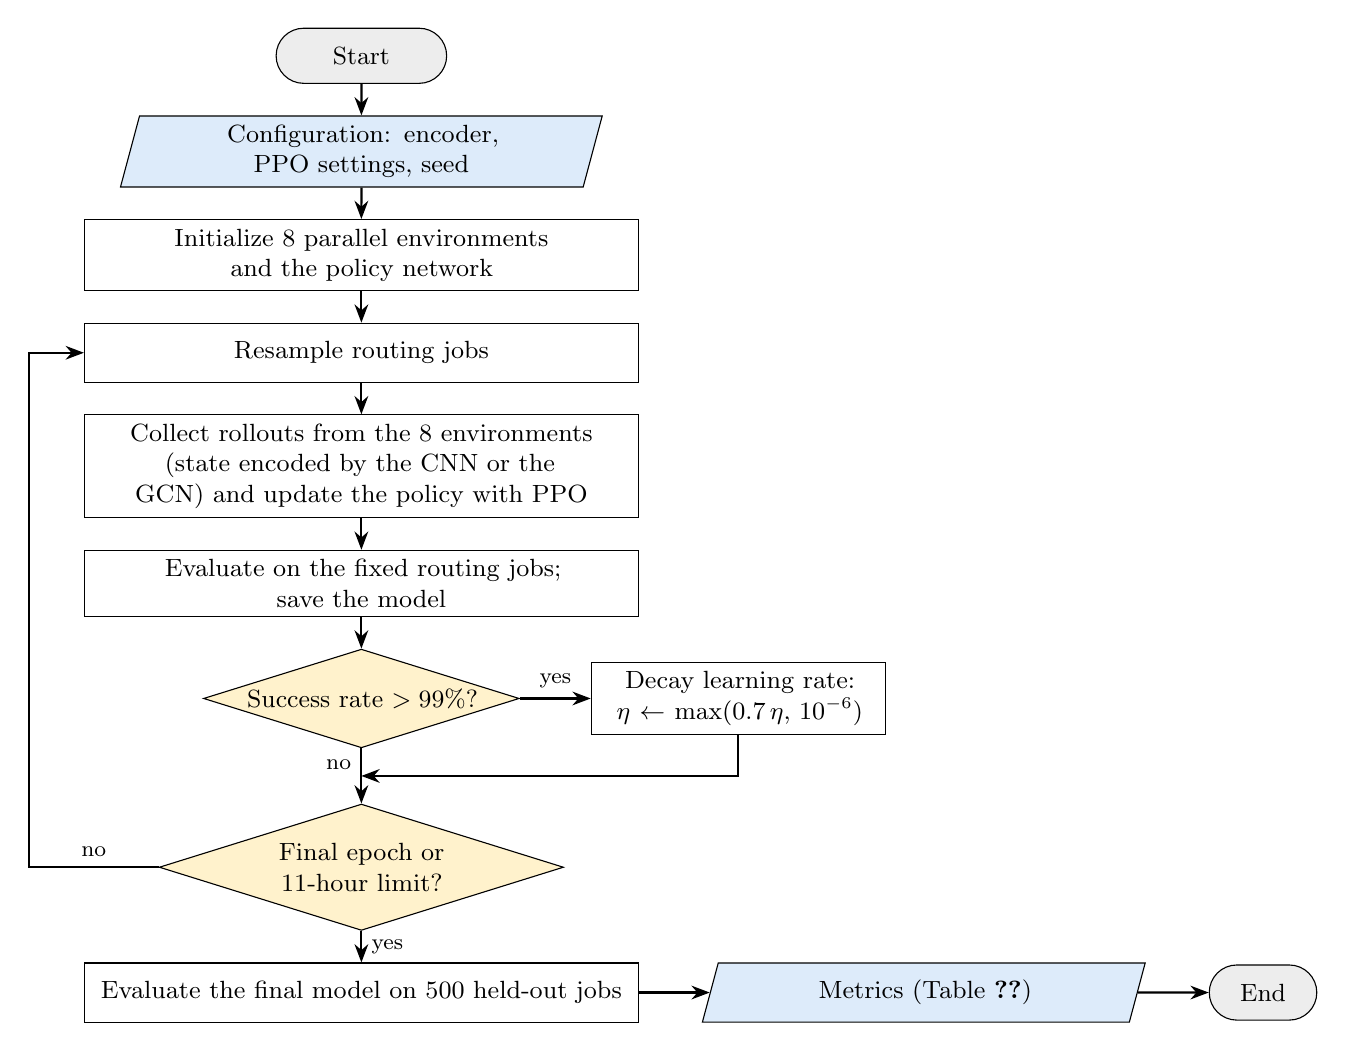
\begin{tikzpicture}[>=Stealth, font=\small, node distance=4mm,
  term/.style={draw, rounded rectangle, fill=same, minimum height=7mm, minimum width=2.4cm},
  proc/.style={draw, rectangle, fill=white, minimum height=7.5mm, text width=6.8cm, align=center,
    execute at begin node={\hyphenpenalty=10000\relax}},
  data/.style={draw, trapezium, trapezium left angle=75, trapezium right angle=105, fill=prop, minimum height=7.5mm, text width=5.4cm, align=center},
  dec/.style={draw, diamond, aspect=3.2, fill=todo, inner sep=1pt, align=center, text width=2.9cm},
  flow/.style={->, thick}]
  \node[term] (start) {Start};
  \node[data, below=of start] (cfg) {Configuration: encoder, PPO settings, seed};
  \node[proc, below=of cfg] (init) {Initialize 8 parallel environments\\ and the policy network};
  \node[proc, below=of init] (jobs) {Resample routing jobs};
  \node[proc, below=of jobs] (train) {Collect rollouts from the 8 environments (state encoded by the CNN or the GCN) and update the policy with PPO};
  \node[proc, below=of train] (eval) {Evaluate on the fixed routing jobs;\\ save the model};
  \node[dec, below=of eval] (d1) {Success rate $>99\%$?};
  \node[proc, right=9mm of d1, text width=3.5cm] (lr) {Decay learning rate:\\ $\eta\leftarrow\max(0.7\,\eta,\,10^{-6})$};
  \node[dec, below=7mm of d1] (d2) {Final epoch or\\ 11-hour limit?};
  \node[proc, below=of d2] (final) {Evaluate the final model on 500 held-out jobs};
  \node[data, right=9mm of final, text width=3.6cm] (out) {Metrics (Table~\ref{tab:metrics})};
  \node[term, right=9mm of out, minimum width=1.6cm] (stop) {End};
  \draw[flow] (start) -- (cfg);
  \draw[flow] (cfg) -- (init);
  \draw[flow] (init) -- (jobs);
  \draw[flow] (jobs) -- (train);
  \draw[flow] (train) -- (eval);
  \draw[flow] (eval) -- (d1);
  \draw[flow] (d1) -- node[above, font=\footnotesize] {yes} (lr);
  \draw[flow] (d1) -- node[left, pos=0.3, font=\footnotesize] {no} (d2);
  \coordinate (join) at ($(d1.south)!0.5!(d2.north)$);
  \draw[flow] (lr.south) |- (join);
  \draw[flow] (d2) -- node[right, font=\footnotesize] {yes} (final);
  \draw[flow] (d2.west) -| node[above, pos=0.25, font=\footnotesize] {no} ([xshift=-7mm]jobs.west) -- (jobs.west);
  \draw[flow] (final) -- (out);
  \draw[flow] (out) -- (stop);
\end{tikzpicture}
\caption{Training and evaluation procedure applied to every configuration.}
\label{fig:flow}
\end{figure}

\begin{table}[H]
\centering\small
\begin{tabularx}{\textwidth}{lL}
\toprule
Metric & Definition \\ \midrule
Success rate & Fraction of jobs in which the droplet reaches the goal within $k_{\max}$ control cycles \\
Routing cycles & Mean, median and standard deviation of control cycles per job; timed-out jobs are counted at $k_{\max}$ \\
Invalid actions per decision & Number of actions that would move the droplet outside the routing zone, divided by the number of decisions \\
Convergence & Environment steps and optimizer steps at the first of three consecutive per-epoch evaluations with a success rate of at least 95\% \\
Computational cost & Wall-clock training time and inference time per decision \\
\bottomrule
\end{tabularx}
\caption{Evaluation metrics.}
\label{tab:metrics}
\end{table}

Table~\ref{tab:plan} lists the compared configurations. The direction-aware
configuration is an ablation that changes only the message-passing layer of
the proposed configuration.

\begin{table}[H]
\centering\small
\begin{tabularx}{\textwidth}{l>{\raggedright\arraybackslash}p{3.6cm}L}
\toprule
Configuration & Purpose & Experiments completed \\ \midrule
CNN--PPO baseline & reference performance & $16\times16$; $30\times30$ (25 epochs; 40 epochs in the chip-size study); chip sizes $30\times30$ to $120\times120$; comparison with the authors' implementation \\
GCN + max pooling & proposed representation & $16\times16$; $30\times30$ (25 epochs) \\
Direction-aware GCN + max pooling & ablation: message-passing layer & $16\times16$; $30\times30$ (25 epochs; 40 epochs in the chip-size study); chip sizes $30\times30$ to $120\times120$ \\
\bottomrule
\end{tabularx}
\caption{Compared configurations and the experiments completed (one seed each;
  three seeds per implementation in the comparison with the authors'
  implementation).}
\label{tab:plan}
\end{table}

\begin{table}[H]
\centering\small
\begin{tabularx}{\textwidth}{lXl}
\toprule
Parameter & Value & Source \\ \midrule
Chips & healthy: no faulty MCs, no initial wear & paper / ref.\ code \\
Degradation $\tau$, $c$ & $\tau\in[0.5,0.7]$, $c\in[500,800]$ per MC & paper \\
Health sensor & $b=2$ bits, $H=\min(\lfloor 4D\rfloor,3)$ & paper (formula) / ref.\ code ($b$) \\
Droplet sizes & $w,h\in\{2,\dots,6\}$, $w/h\in[0.8,1.25]$ (9 sizes) & paper \\
Job sampling & stratified start and goal positions (edge weight 0.2); start $\neq$ goal & paper / ref.\ code \\
Routing zone & bounding box of start and goal $\pm3$ MCs & reference code \\
Reward & $+0.5\,\Delta d$ if closer, else $0.8\,\Delta d-1$; $+100$ at goal; $-1$ invalid & reference code \\
$k_{\max}$ & $\alpha(W_h+H_h)$ with $\alpha=1$; episodes cut off at $k_{\max}$ are truncated (value bootstrapped) & paper ($\alpha$ and truncation assumed) \\
Observation & CNN: $30\times30$, larger chips resampled by area averaging ($16\times16$ study: native $16\times16$); GCN: native $W\times H$ grid & paper / methodology \\
PPO & 8 envs; 64 steps; minibatch 32; 4 epochs; $\gamma=0.99$; $\lambda=0.95$; entropy coefficient 0.01; clip range 0.2 (policy and value); gradient-norm limit 0.5 & paper / ref.\ code \\
Value-loss coefficient & 0.25 ($30\times30$ and larger); 0.5 ($16\times16$ study) & ref.\ code / assumed \\
Learning rate & $\eta_0=3.5\times10^{-4}$; $\times0.7$ when evaluation success $>99\%$; floor $10^{-6}$; square-root decay within an epoch & paper / ref.\ code \\
Baseline CNN & $30\times30$ and larger: 64/128/128 filters, FC 256; $16\times16$ study: 32/64/64 filters, FC 128, native input & paper / ref.\ code \\
Epoch / evaluation & $2^{14}$ steps per epoch; after each epoch, 500 fixed evaluation jobs; $30\times30$: 25 and 40 epochs; chip-size study: 40 epochs, stopped before any epoch ending after 11\,h; $16\times16$ study: $2^{13}$ steps, 300 jobs, 40 epochs & paper / assumed \\
Held-out evaluation & final model, deterministic policy, 500 jobs from a separate seed, identical for every configuration & assumed \\
Graph connectivity & 8 neighbours, both directions, no edge attributes & methodology \\
GCN & 3 layers, $d=64$, ReLU & assumed \\
Direction-aware GCN & 3 layers, $d=64$, ReLU; separate weights for the node and each of the 8 directions & assumed \\
Readout & global max pooling & methodology \\
Seeds / repeats & 1 per configuration; 3 per implementation in the comparison with the authors' implementation; 5 planned, as in the paper & assumed / paper \\
\bottomrule
\end{tabularx}
\caption{Implementation parameters and their source: \cite{elfar2023} (paper),
  \cite{elfarcode} (reference code) and the project's GCN methodology
  specification (methodology). \textbf{Assumed} values are either not
  specified in \cite{elfar2023} or are subject to further study.}
\label{tab:params}
\end{table}

% ================================================================= 6 PLATFORM
\section{Simulation Platform and Requirements}\label{sec:platform}

All experiments are conducted in simulation. The MEDA simulator models the
chip grid, per-MC degradation and health sensing, the droplet state,
stochastic health-dependent movement, the action semantics, the reward and
episode termination. It is implemented as a Gymnasium environment
\cite{towers2024}, and training uses the PPO implementation of
Stable-Baselines3 \cite{raffin2021}. Figure~\ref{fig:loop} shows the
interaction of the components. The state encoder is interchangeable: the CNN
or the GCN is selected in the configuration file. Table~\ref{tab:platform}
lists the hardware and software used.

\begin{figure}[H]
\centering
\resizebox{0.95\textwidth}{!}{%
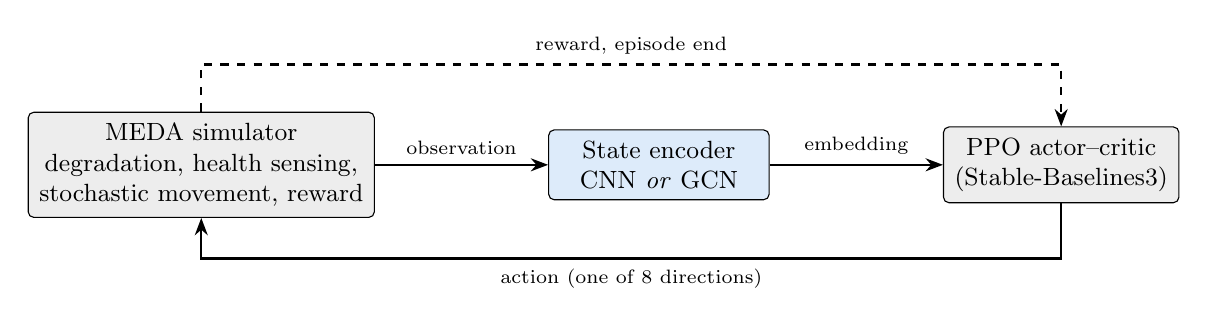
\begin{tikzpicture}[node distance=5mm and 22mm]
  \node[blk=same, minimum width=3.4cm] (sim) {MEDA simulator\\degradation, health sensing,\\stochastic movement, reward};
  \node[blk=prop, right=of sim, minimum width=2.8cm] (enc) {State encoder\\CNN \emph{or} GCN};
  \node[blk=same, right=of enc, minimum width=2.8cm] (ppo) {PPO actor--critic\\(Stable-Baselines3)};
  \draw[arr] (sim) -- node[above, font=\scriptsize]{observation} (enc);
  \draw[arr] (enc) -- node[above, font=\scriptsize]{embedding} (ppo);
  \draw[arr] (ppo.south) -- ++(0,-0.7) -| node[pos=0.25, below, font=\scriptsize]{action (one of 8 directions)} (sim.south);
  \draw[arr, dashed] (sim.north) -- ++(0,0.6) -| node[pos=0.25, above, font=\scriptsize]{reward, episode end} (ppo.north);
\end{tikzpicture}}
\caption{Agent--environment loop and software architecture.}
\label{fig:loop}
\end{figure}

\begin{table}[H]
\centering\small
\begin{tabularx}{\textwidth}{lLLL}
\toprule
& $16\times16$ study (CPU) & $30\times30$ and chip-size studies (GPU) & Authors' implementation (CPU) \\ \midrule
Platform & cloud container & Kaggle notebook sessions & Kaggle notebook sessions \\
Operating system & Ubuntu 24.04.4 LTS (Linux 6.18) & Linux & Linux \\
CPU & Intel Xeon @ 2.10\,GHz, 4 logical cores & 4 logical cores & -- \\
GPU & none & NVIDIA Tesla T4 (14.6\,GiB), one per run & none \\
Python & 3.11.15 & 3.12 (25-epoch runs); 3.13 (all later runs) & 3.7 \\
Learning framework & PyTorch 2.14.0 (CPU) & PyTorch of the session image & TensorFlow 1.15.5 \\
RL libraries & Stable-Baselines3 2.9.0, Gymnasium 1.3.0 & Stable-Baselines3 ($\geq$2.2), Gymnasium ($\geq$0.29), installed per session & Stable Baselines 2.10.1, Gym 0.18.0 \\
Other libraries & NumPy 2.4.6, OpenCV 5.0.0, pandas 3.0.6, matplotlib 3.11.2, PyYAML 6.0.1, pytest 9.1.1 & same package requirements & -- \\
Graph library & none; message passing in plain PyTorch & same & -- \\
\bottomrule
\end{tabularx}
\caption{Platforms used. Library versions on the GPU platform were those
  current at the time of each run and were not recorded.}
\label{tab:platform}
\end{table}

% ================================================================= 7 PRELIMINARY RESULTS
\section{Preliminary Results}\label{sec:results}

All results in this section come from a single training seed per
configuration, except the comparison with the authors' implementation in
Section~\ref{sec:refcheck}, which uses three seeds per implementation, and
all chips are healthy. Section~\ref{sec:res16} compares the three
configurations on $16\times16$ chips and Section~\ref{sec:res30} on
$30\times30$ chips; Section~\ref{sec:sizes} compares the baseline with the
direction-aware GCN on chips of $30\times30$ to $120\times120$ MCs.

\subsection{Results on $16\times16$ chips}\label{sec:res16}
Table~\ref{tab:results} and Figure~\ref{fig:curves} report the comparison of
the three configurations on $16\times16$ chips.

\begin{table}[H]
\centering\small
\begin{tabular}{lrrrrr}
\toprule
Method & Success & Mean & Invalid actions & Steps to & Encoder \\
 & (\%) & cycles$^{*}$ & per decision & convergence & parameters \\ \midrule
CNN--PPO (baseline) & 96.2 & 5.94 & 0.12 & 221\,k & 2.15\,M \\
GCN + max pooling & 4.0 & 25.06 & 0.88 & not reached & 8.6\,k \\
Direction-aware GCN + max pooling & \textbf{99.4} & \textbf{4.89} & \textbf{0.004} & \textbf{74\,k} & 76\,k \\
\bottomrule
\end{tabular}
\caption{Preliminary comparison on healthy $16\times16$ chips (one seed,
  327\,680 environment steps per configuration, the same 500 held-out jobs for
  every configuration). The $16\times16$ baseline uses the smaller CNN of the
  reference implementation \cite{elfarcode}. $^{*}$Timed-out jobs are counted at $k_{\max}$
  cycles.}
\label{tab:results}
\end{table}

\begin{figure}[H]
\centering
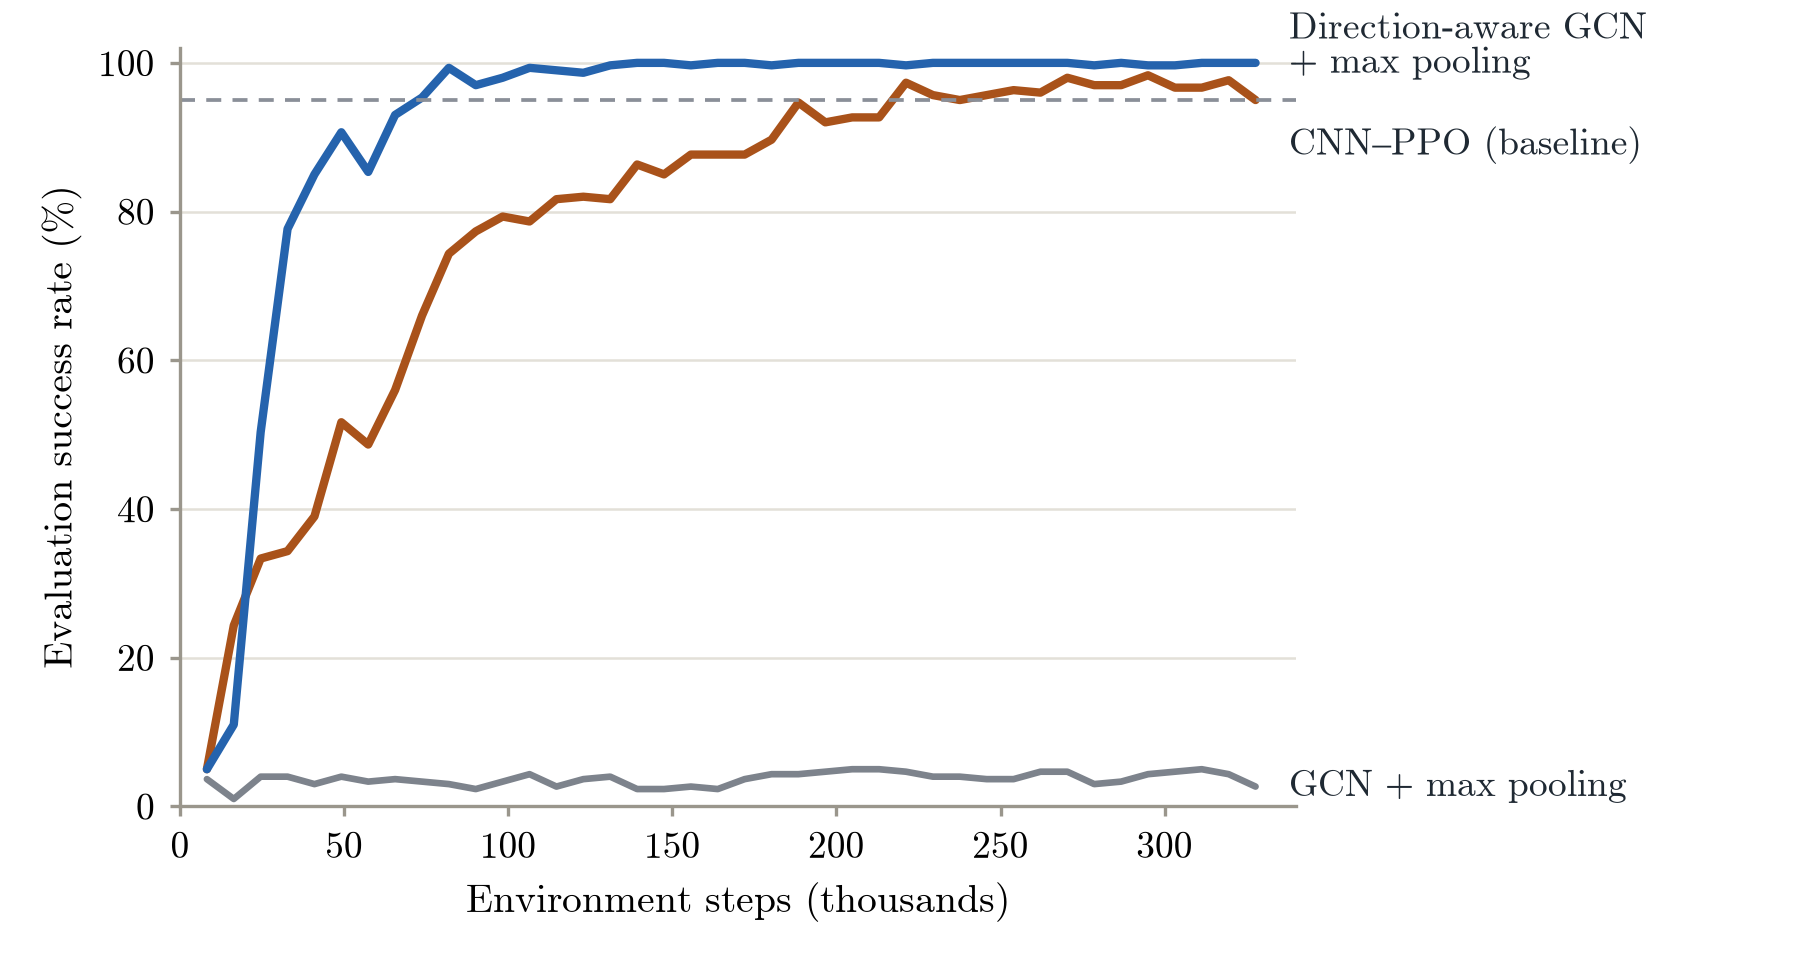
\includegraphics[width=0.8\textwidth]{figures/learning_curves.png}
\caption{Evaluation success rate during training on $16\times16$ chips
  (one seed; per-epoch evaluation on 300 jobs). The dashed line marks the 95\%
  convergence threshold.}
\label{fig:curves}
\end{figure}

The GCN with global max pooling did not learn a routing policy within the
training budget: its success rate on the held-out jobs was 4.0\%, no per-epoch
evaluation exceeded 5.0\%, and it made 0.88 invalid actions per decision. The
GCN aggregates neighbour messages with weights that do not depend on
direction; consequently, as shown in Section~\ref{sec:method}, a routing job
and its mirror images and rotations receive the same graph embedding, and the
policy receives identical inputs for jobs that require different actions.

Replacing only the message-passing layer with the direction-aware graph
convolution of Section~\ref{sec:method} removes this symmetry. The resulting
configuration achieved a success rate of 99.4\% at 4.89 mean cycles and
converged within 74\,k environment steps, compared with 96.2\%, 5.94 cycles
and 221\,k steps for the CNN--PPO baseline, while using 76\,k encoder
parameters instead of 2.15\,M. These results were obtained with a single seed
on a reduced problem size; the comparison at the chip size of the base paper
follows.

\subsection{Results on $30\times30$ chips}\label{sec:res30}
Table~\ref{tab:results30} reports the comparison on $30\times30$ chips after
25 epochs for all three configurations and after 40 epochs for the baseline
and the direction-aware GCN; Figure~\ref{fig:curves30} shows the learning
curves.

\begin{table}[H]
\centering\small
\begin{tabular}{lrrrrr}
\toprule
Method & Success & Mean & Invalid actions & Steps to & Encoder \\
 & (\%) & cycles$^{*}$ & per decision & convergence & parameters \\ \midrule
\multicolumn{6}{l}{\emph{25 epochs (409\,600 environment steps)}} \\
CNN--PPO (baseline) & 70.2 & 19.54 & 0.21 & not reached & 29.7\,M \\
GCN + max pooling & 2.8 & 38.09 & 0.88 & not reached & 8.6\,k \\
Direction-aware GCN + max pooling & \textbf{100.0} & \textbf{9.87} & \textbf{0.000} & \textbf{147\,k} & 76\,k \\ \midrule
\multicolumn{6}{l}{\emph{40 epochs (655\,360 environment steps)}} \\
CNN--PPO (baseline) & 87.4 & 14.52 & 0.10 & not reached & 29.7\,M \\
Direction-aware GCN + max pooling & \textbf{100.0} & \textbf{9.84} & \textbf{0.000} & \textbf{147\,k} & 76\,k \\
\bottomrule
\end{tabular}
\caption{Comparison on healthy $30\times30$ chips (one seed per run, the same
  500 held-out jobs for every configuration). The baseline uses the CNN of
  Table~I in \cite{elfar2023}. GCN + max pooling was not trained for 40
  epochs. $^{*}$Timed-out jobs are counted at $k_{\max}$ cycles.}
\label{tab:results30}
\end{table}

\begin{figure}[H]
\centering
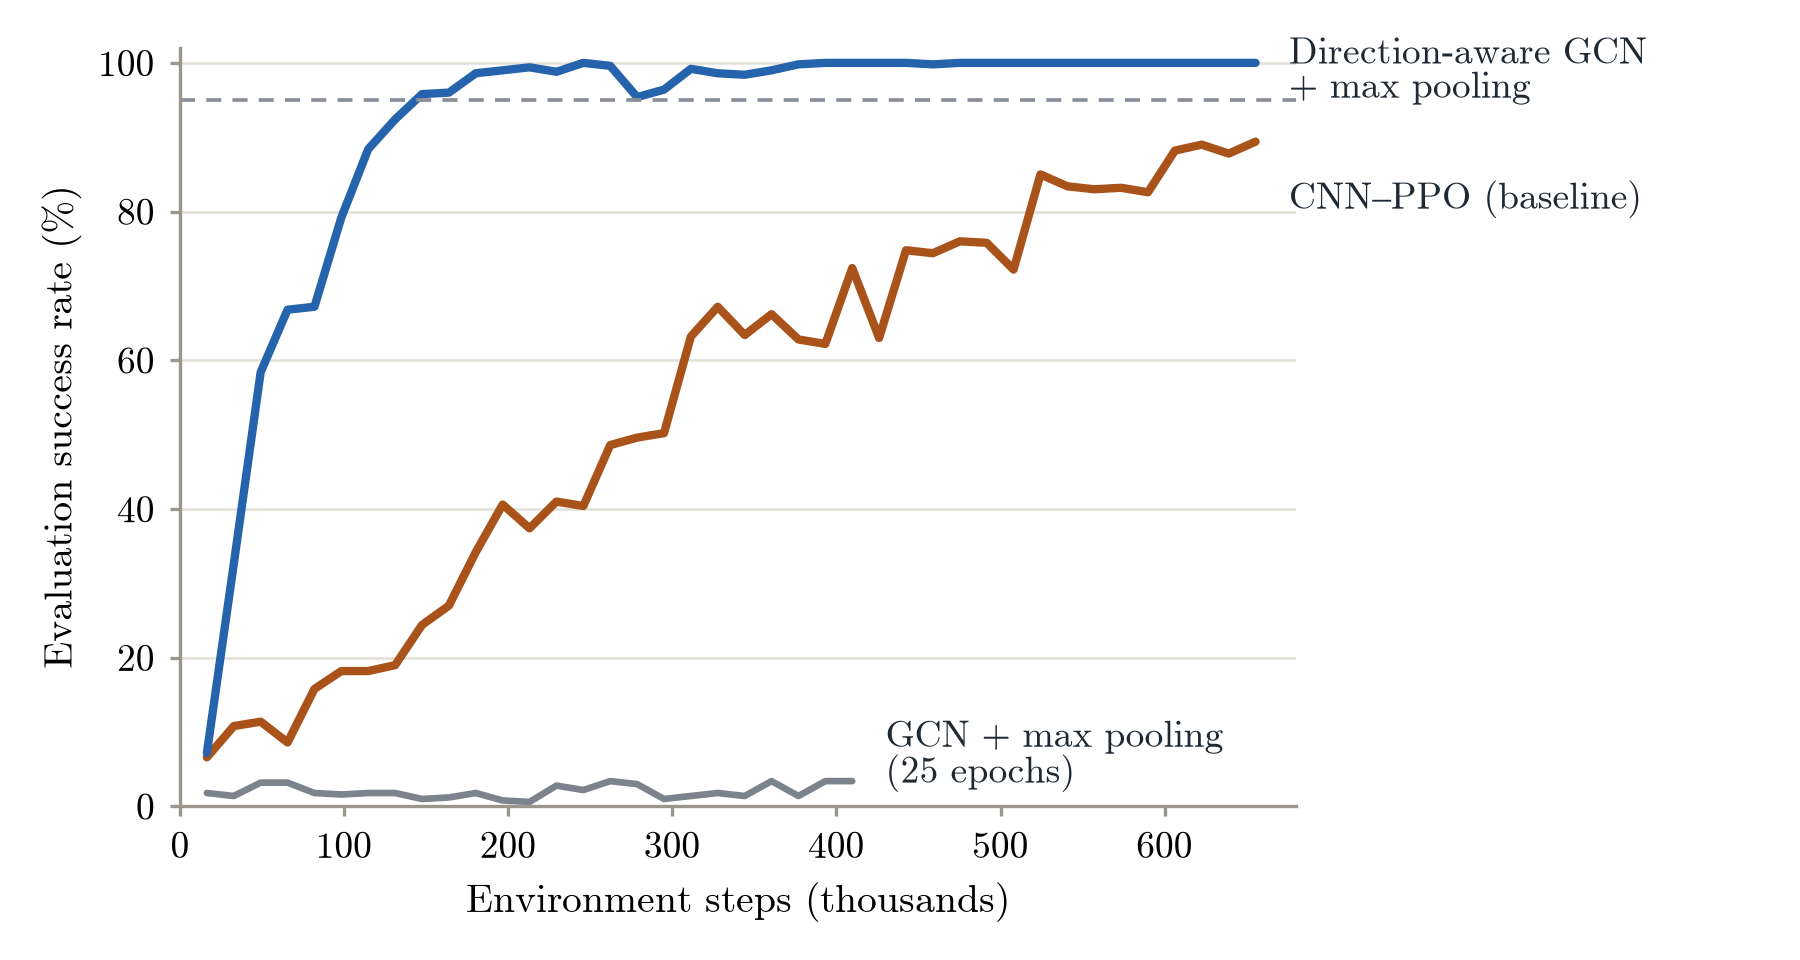
\includegraphics[width=0.8\textwidth]{figures/learning_curves_30x30.png}
\caption{Evaluation success rate during training on $30\times30$ chips (one
  seed; per-epoch evaluation on 500 jobs): the baseline and the
  direction-aware GCN over 40 epochs, GCN + max pooling over its 25 epochs. The
  dashed line marks the 95\% convergence threshold.}
\label{fig:curves30}
\end{figure}

The $30\times30$ results agree with the $16\times16$ study. The GCN with
global max pooling again failed to learn a routing policy (2.8\% success,
0.88 invalid actions per decision); the trained model selected the same
action, east, for all 500 held-out jobs, which is consistent with the
symmetry argument of Section~\ref{sec:method}. The direction-aware GCN routed
all 500 held-out jobs and met the convergence criterion after 147\,k
environment steps (epoch 9) in both runs.

The CNN--PPO baseline met the convergence criterion in neither run. After 25
epochs it reached 70.2\% success at 19.54 cycles; its per-epoch evaluation
peaked at 73.8\% in epoch 23 and was 67.2\% in the last two epochs. A
separate 40-epoch run, trained with the same seed, reached 87.4\% held-out
success at 14.52 cycles, with a best per-epoch evaluation of 89.4\% in the
final epoch, so the baseline's results reflect the fixed training budget
rather than its final performance.
On the same held-out jobs, the direction-aware GCN solved all 63 jobs that the
baseline failed after 40 epochs, while the baseline solved none that the GCN
failed (exact McNemar test, $p=2.2\times10^{-19}$); on the 437 jobs that both
solved, the GCN needed 9.25 cycles on average and the baseline 11.08. The
baseline's failures concentrate on the smallest droplets, which advance by one
MC per step: its success rate was 64.3\% for $2\times2$ droplets, 75.0\% for
$3\times3$ droplets and 92.5\% for the larger sizes. With 40 epochs, training
took 40 and 45 minutes for the baseline and the direction-aware configuration
on one Tesla T4 GPU. Retrained with the same seed in a later software
environment, the baseline did not repeat its per-epoch results (72.4\% instead
of 67.2\% at epoch 25), whereas the direction-aware GCN repeated them exactly.

\subsection{Chip-size study}\label{sec:sizes}
The baseline and the direction-aware GCN were trained from scratch on healthy
chips of $30\times30$, $50\times50$, $60\times60$, $100\times100$ and
$120\times120$ MCs, each with a budget of 40 epochs of $2^{14}$ steps and
otherwise unchanged settings; GCN + max pooling was not included. Elfar et
al.\ \cite{elfar2023} also evaluate $60\times60$ and $120\times120$ chips, but
train them by transfer learning from smaller chips, so their results are not
directly comparable. Table~\ref{tab:sizes} and Figure~\ref{fig:sizes} report
the results.

\begin{table}[H]
\centering\small
\setlength{\tabcolsep}{3pt}
\begin{tabular}{llrrrrrr}
\toprule
Chip & Method & Success & Mean & Invalid actions & Steps to & Epochs & Seconds \\
 & & (\%) & cycles$^{*}$ & per decision & convergence & trained & per epoch \\ \midrule
$30\times30$ & CNN--PPO & 87.4 & 14.52 & 0.10 & not reached & 40 & 59 \\
 & Direction-aware GCN & \textbf{100.0} & \textbf{9.84} & \textbf{0.000} & \textbf{147\,k} & 40 & 67 \\ \midrule
$50\times50$ & CNN--PPO & 44.6 & 41.04 & 0.21 & not reached & 40 & 66 \\
 & Direction-aware GCN & \textbf{100.0} & \textbf{16.71} & \textbf{0.000} & \textbf{213\,k} & 40 & 204 \\ \midrule
$60\times60$ & CNN--PPO & 27.8 & 53.48 & 0.45 & not reached & 40 & 73 \\
 & Direction-aware GCN & \textbf{99.6} & \textbf{20.94} & \textbf{0.001} & \textbf{213\,k} & 40 & 264 \\ \midrule
$100\times100$ & CNN--PPO & 15.6 & 86.47 & 0.31 & not reached & 40 & 94 \\
 & Direction-aware GCN & \textbf{99.8} & \textbf{34.31} & \textbf{0.000} & \textbf{459\,k} & 34$^{\dagger}$ & 1\,156 \\ \midrule
$120\times120$ & CNN--PPO & 10.2 & 108.61 & 0.39 & not reached & 40 & 112 \\
 & Direction-aware GCN & \textbf{89.2} & \textbf{61.90} & \textbf{0.030} & not reached & 21$^{\dagger}$ & 1\,852 \\
\bottomrule
\end{tabular}
\caption{Chip-size study on healthy chips (one seed per run, the same 500
  held-out jobs for both methods at each size). The baseline observes every
  chip resampled to $30\times30$; the GCN operates on the native grid. Seconds
  per epoch: mean wall-clock time of $2^{14}$ training steps and the per-epoch
  evaluation on one Tesla T4 GPU. $^{*}$Timed-out jobs are counted at
  $k_{\max}$ cycles. $^{\dagger}$Training stopped by the 11-hour limit.}
\label{tab:sizes}
\end{table}

\begin{figure}[H]
\centering
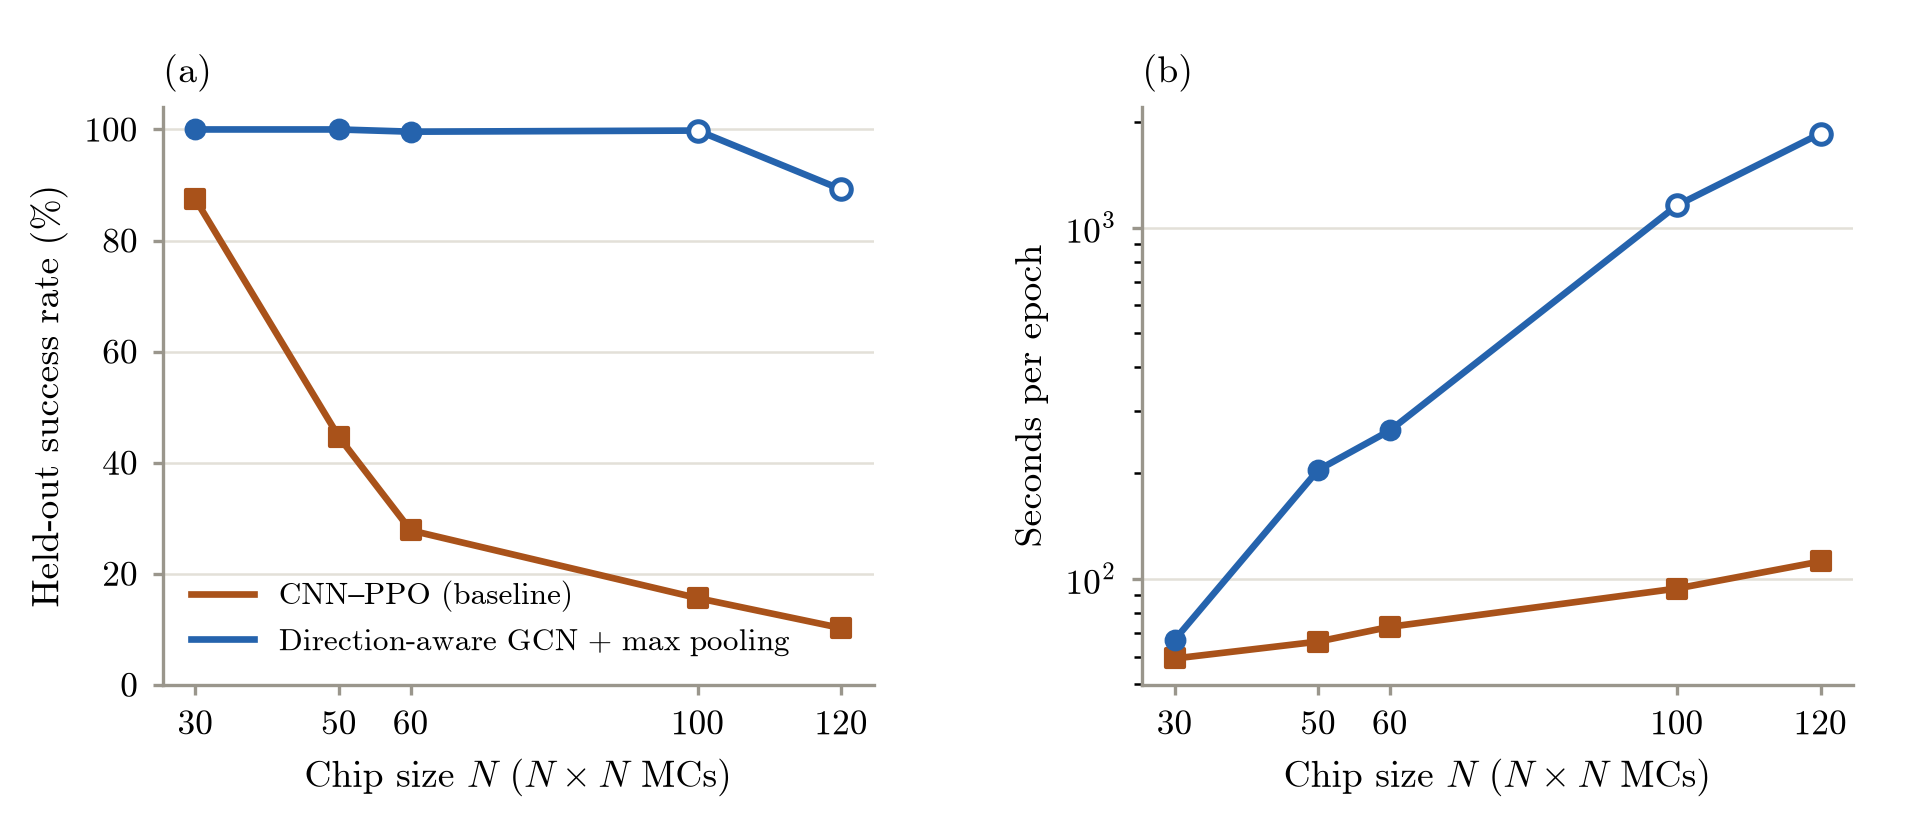
\includegraphics[width=0.95\textwidth]{figures/chip_size.png}
\caption{Chip-size study (one seed per run): (a) success rate on the 500
  held-out jobs; (b) mean seconds per training epoch, on a logarithmic scale.
  The baseline did not meet the convergence criterion at any size.
  Hollow markers: runs stopped by the 11-hour limit after 34 ($100\times100$)
  and 21 ($120\times120$) of 40 epochs.}
\label{fig:sizes}
\end{figure}

The success rate of the baseline decreased from 87.4\% on $30\times30$ chips
to 10.2\% on $120\times120$ chips, and it did not meet the convergence
criterion at any size. The direction-aware GCN routed at least 99.6\% of the
held-out jobs on chips of up to $100\times100$ MCs and converged at each of
these sizes, after 213\,k environment steps on $50\times50$ and $60\times60$
chips and 459\,k on $100\times100$ chips. At every size, the jobs solved by
only one of the two methods were almost all solved by the GCN (exact McNemar
test, $p\leq2.2\times10^{-19}$ at every size).

The computation of the direction-aware GCN grows with the number of MCs,
whereas the baseline network always processes a $30\times30$ input. The mean
time per epoch of the GCN grew from 67\,s on $30\times30$ chips to 1\,852\,s on
$120\times120$ chips, against 59 to 112\,s for the baseline, and its
multiply--accumulate operations per forward pass exceed those of the baseline
CNN (230\,M) from about $55\times55$ MCs. On $100\times100$ and $120\times120$
chips, the 11-hour limit stopped the GCN after 34 and 21 of its 40 epochs, so
it received fewer environment steps than the baseline; at those epochs, the
per-epoch success rate of the baseline was 6.4\% and 2.6\%. On $120\times120$
chips the GCN had not met the convergence criterion when its training stopped
(per-epoch success rate 86.4\% in its last epoch).

\subsection{Comparison with the authors' original implementation}\label{sec:refcheck}
To check our implementation of the CNN--PPO baseline, it and the authors'
original implementation \cite{elfarcode} (unmodified, at commit
\texttt{1667016}, in its original software environment) were trained with the
settings of the authors' logged $30\times30$ training run for 40 epochs of
$2^{14}$ steps, with three seeds each; after every epoch, the deterministic
policy was evaluated on 500 routing jobs. These settings differ from those of
the other experiments in this report: five droplet sizes ($4\times4$ to
$6\times6$), $k_{\max}=W+H$, and collision marks in the observation. The
original implementation at this commit uses a smaller CNN (32, 64 and 64
filters, FC 128; 7.43\,M parameters) and multiplies the learning rate by 0.7
after an epoch with 100\% success. Our first runs used the Table~I network and
the factor 0.5 of the authors' log; a second set of runs used the network and
decay factor of the original implementation, although none of these runs
reached 100\% success in an epoch, so the decay was never applied.
Table~\ref{tab:reference} and
Figure~\ref{fig:reference} report the results.

\begin{table}[H]
\centering\small
\begin{tabular}{lrrrr}
\toprule
Implementation & First epoch & Convergence & Final & Final \\
 & $\geq$95\% success & epoch & success (\%) & cycles \\ \midrule
Authors' implementation \cite{elfarcode} & $25.7\pm3.1$ & $25.7\pm3.1$ & $99.81\pm0.15$ & $7.95\pm0.61$ \\
Ours, Table~I CNN & $20.3\pm0.6$ & $23.3\pm1.5$ & $99.05\pm0.26$ & $8.42\pm0.14$ \\
Ours, CNN and decay of the original & $18.7\pm1.5$ & $20.7\pm3.5$ & $98.64\pm0.28$ & $8.70\pm0.20$ \\
\bottomrule
\end{tabular}
\caption{Comparison with the authors' original implementation under the
  settings of their logged $30\times30$ run (mean $\pm$ standard deviation over
  three seeds). Convergence: first of three consecutive evaluations at or
  above 95\%. Final values: mean over epochs 36--40.}
\label{tab:reference}
\end{table}

\begin{figure}[H]
\centering
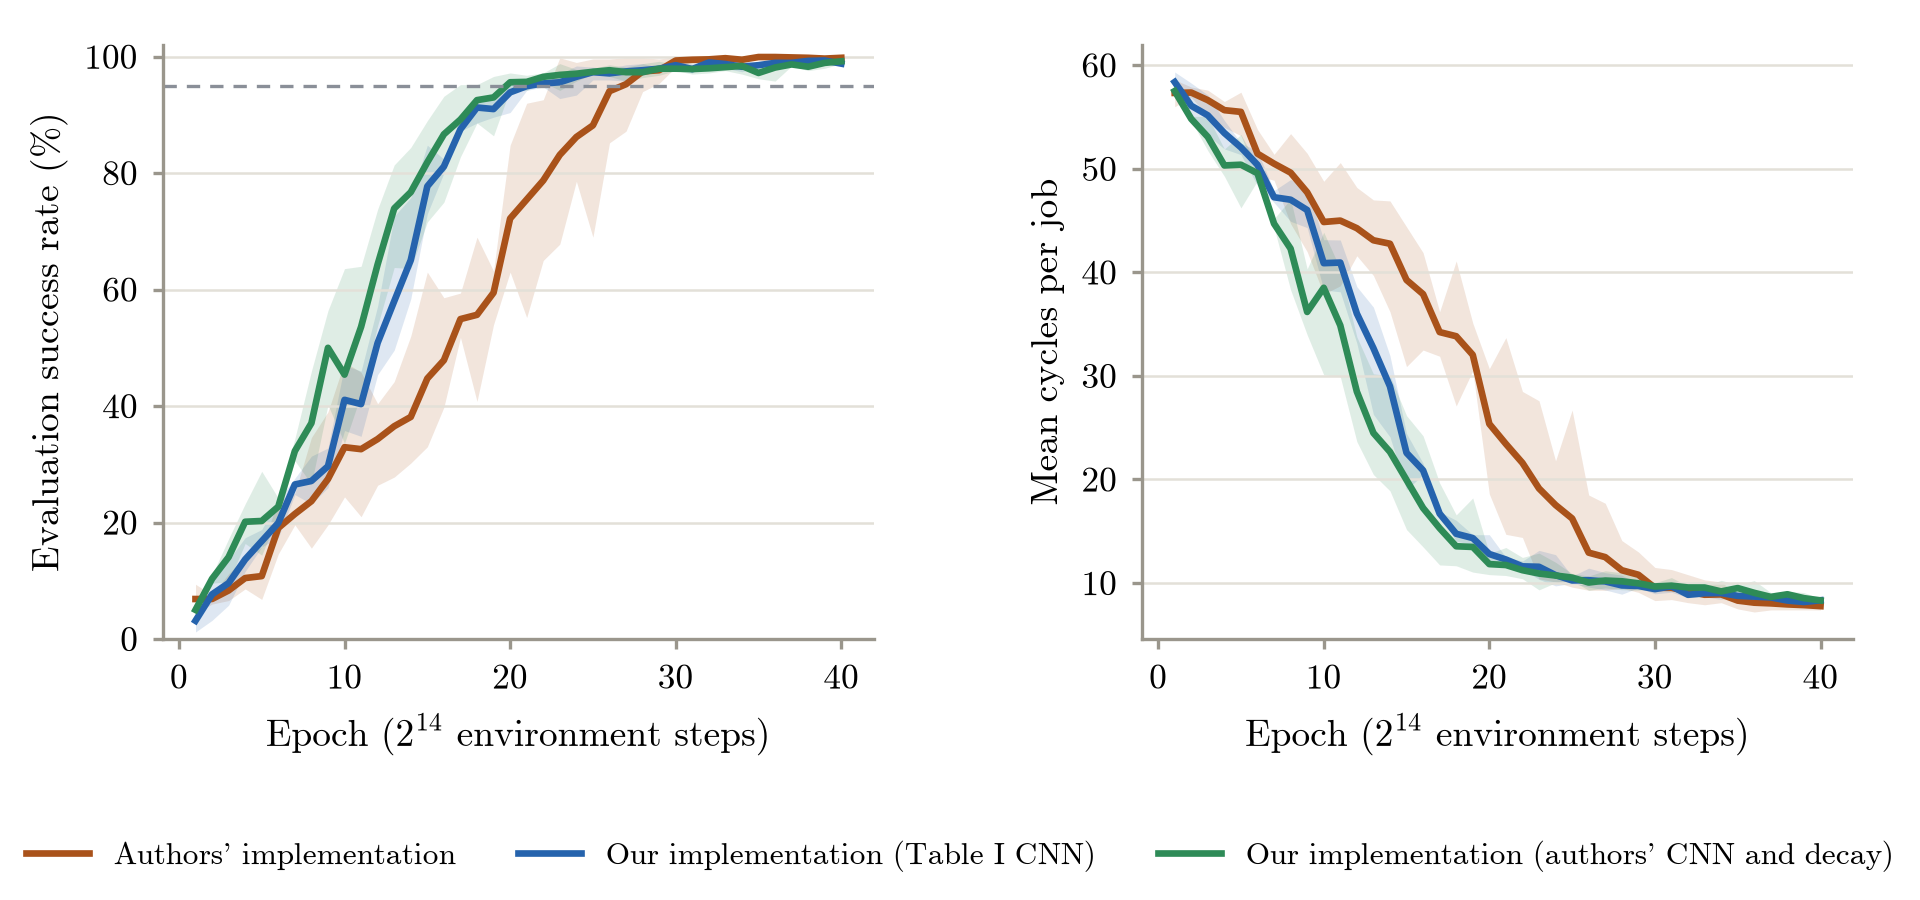
\includegraphics[width=0.95\textwidth]{figures/reference_test.png}
\caption{Per-epoch evaluation success rate (left) and mean cycles (right) of
  the authors' original implementation and of the two variants of our
  implementation (three seeds each; line: mean, band: minimum to maximum).
  The dashed line marks the 95\% convergence threshold.}
\label{fig:reference}
\end{figure}

All runs reached a per-epoch success rate of 99.4--100\%. Our implementation reached
95\% success earlier, in epoch 20.3 and 18.7 on average against 25.7 (Welch's
$t$-test, $p=0.089$ and $p=0.039$), and met the convergence criterion in
epoch 23.3 and 20.7 against 25.7 ($p=0.32$ and $p=0.14$). Its final success
rate was 0.8 and 1.2 percentage points lower ($p=0.019$ and $p=0.007$), and
its final cycles were 8.42 and 8.70 against 7.95 ($p=0.31$ and $p=0.16$).
After Holm correction over the four metrics, only the lower final success
rate of the second set of runs remains significant ($p=0.028$; all other
adjusted values are 0.077 or more). Using the network and decay factor of the
original implementation made no detectable difference to our implementation
($p\geq0.13$ for all four metrics). The remaining differences
between the implementations include the evaluation protocol (a fixed set of
500 jobs here; fresh jobs, counting the first 500 to finish, in the original),
the treatment of timed-out episodes and the PPO implementations. With three
seeds per implementation, the comparison gives no indication that our
implementation of the baseline learns more slowly than the original. The slow
learning of the baseline in Sections~\ref{sec:res30} and \ref{sec:sizes} is
therefore unlikely to stem from our implementation; it coincides with the
harder job distribution of the paper's settings (nine droplet sizes, including
$2\times2$ and $3\times3$, and a $k_{\max}$ based on the routing zone),
although the contribution of each setting has not been isolated.

\subsection{Limitations}
\begin{itemize}
  \item Every comparison of the configurations uses a single training seed;
        repeated runs with five seeds are planned.
  \item The baseline did not meet the convergence criterion on any chip of
        $30\times30$ MCs or more, so the comparisons hold for the stated
        training budgets only.
  \item On chips larger than $30\times30$, the baseline observes a resampled
        chip and the GCN the native grid. The direction-aware GCN also
        differs from the baseline CNN in its readout (global max pooling
        instead of a fully connected layer), its width and its embedding size,
        so the comparison does not separate the effect of the graph
        representation from these factors.
  \item In Sections~\ref{sec:res16}--\ref{sec:sizes}, the learning-rate decay of
        Section~\ref{sec:method} was triggered only for the direction-aware
        GCN, the only configuration that exceeded 99\% success.
  \item All chips are healthy, so the sensed health of almost every MC stays
        at its maximum level during an episode, the health channel acts
        essentially as a mask of the routing zone, and degradation-aware
        routing is not yet exercised.
  \item Each chip size was trained from scratch with the same budget, unlike
        the transfer learning of \cite{elfar2023}, and the 11-hour limit
        reduced the budget of the GCN on the two largest chips.
\end{itemize}

% ================================================================= 8 CONCLUSION
\section{Conclusion and Future Work}\label{sec:conclusion}

This work addresses reliable droplet routing on MEDA biochips, where
electrode degradation renders droplet movement stochastic and routing must
account for the sensed health of the micro-electrodes. The MC graph
representation and the GCN--PPO pipeline have been implemented, and a
controlled comparison with the CNN--PPO method of Elfar et al.\
\cite{elfar2023} has been carried out on healthy chips of $16\times16$ to
$120\times120$ MCs; a training comparison with the authors' original
implementation gave no indication that our implementation of the baseline
learns more slowly. In these single-seed comparisons, the isotropic GCN with
global max pooling did not learn to route, which is explained by its invariance
to the symmetries of the chip, whereas the direction-aware GCN with global max
pooling, equivalent to a fully convolutional network with global max pooling,
exceeded the CNN baseline in success rate and routing cycles at every chip
size within the same or a smaller number of environment steps, with 393 times
fewer encoder parameters than the Table~I CNN (100\% against 87.4\% success on $30\times30$ chips after
40 epochs, and 99.8\% against 15.6\% on $100\times100$ chips). The baseline did
not converge within the budget at any size of $30\times30$ MCs or more, so
these results hold for the stated budgets. They indicate that the
message-passing layer must be sensitive to direction; the cost of the GCN,
however, grows with the number of MCs, so that on the largest chips its
training was limited by time rather than by the number of environment steps.\\
Future work will repeat the comparisons with five seeds per configuration;
separate the effects of the graph representation, the readout and the
observation resolution with additional controls; evaluate zero-shot transfer
across chip sizes, which the size-independent weights of the GCN permit
without resizing the observations; and assess performance on chips with
injected faults, where degradation-aware routing matters, and on the COVID-19
bioassay benchmarks.

% ================================================================= REFERENCES
\phantomsection\label{sec:refs}
\begin{thebibliography}{99}\small
\bibitem{elfar2023} M.~Elfar, Y.-C.~Chang, H.~H.-Y.~Ku, T.-C.~Liang, K.~Chakrabarty and M.~Pajic, ``Deep reinforcement learning-based approach for efficient and reliable droplet routing on MEDA biochips,'' \emph{IEEE Trans.\ Computer-Aided Design of Integrated Circuits and Systems}, vol.~42, no.~4, pp.~1212--1222, 2023, doi:10.1109/TCAD.2022.3194808.
\bibitem{elfarcode} M.~Elfar, ``MEDA,'' public reference implementation, GitHub repository \url{https://github.com/melfar87/MEDA}.
\bibitem{elfar2022date} M.~Elfar, T.-C.~Liang, K.~Chakrabarty and M.~Pajic, ``Adaptive droplet routing for MEDA biochips via deep reinforcement learning,'' in \emph{Proc.\ Design, Automation \& Test in Europe (DATE)}, 2022, pp.~640--645.
\bibitem{elfar2021date} M.~Elfar, T.-C.~Liang, K.~Chakrabarty and M.~Pajic, ``Formal synthesis of adaptive droplet routing for MEDA biochips,'' in \emph{Proc.\ DATE}, 2021, pp.~324--329.
\bibitem{elfar2022tcad} M.~Elfar, T.-C.~Liang, K.~Chakrabarty and M.~Pajic, ``Formal synthesis of adaptive droplet routing for MEDA biochips,'' \emph{IEEE Trans.\ Computer-Aided Design of Integrated Circuits and Systems}, vol.~41, no.~8, pp.~2504--2517, 2022.
\bibitem{liang2020} T.-C.~Liang, Z.~Zhong, Y.~Bigdeli, T.-Y.~Ho, K.~Chakrabarty and R.~Fair, ``Adaptive droplet routing in digital microfluidic biochips using deep reinforcement learning,'' in \emph{Proc.\ Int.\ Conf.\ Machine Learning (ICML)}, PMLR vol.~119, 2020, pp.~6050--6060.
\bibitem{liang2021} T.-C.~Liang, J.~Zhou, Y.-S.~Chan, T.-Y.~Ho, K.~Chakrabarty and C.-Y.~Lee, ``Parallel droplet control in MEDA biochips using multi-agent reinforcement learning,'' in \emph{Proc.\ ICML}, PMLR vol.~139, 2021, pp.~6588--6599.
\bibitem{pollack2000} M.~G.~Pollack, R.~B.~Fair and A.~D.~Shenderov, ``Electrowetting-based actuation of liquid droplets for microfluidic applications,'' \emph{Applied Physics Letters}, vol.~77, no.~11, pp.~1725--1726, 2000.
\bibitem{chakrabarty2006} K.~Chakrabarty and F.~Su, \emph{Digital Microfluidic Biochips: Synthesis, Testing, and Reconfiguration Techniques}. CRC Press, 2006.
\bibitem{wang2011} G.~Wang, D.~Teng and S.-K.~Fan, ``Digital microfluidic operations on micro-electrode dot array architecture,'' \emph{IET Nanobiotechnology}, vol.~5, no.~4, pp.~152--160, 2011.
\bibitem{li2017} Z.~Li, K.~Y.-T.~Lai, P.-H.~Yu, K.~Chakrabarty, T.-Y.~Ho and C.-Y.~Lee, ``Droplet size-aware high-level synthesis for micro-electrode-dot-array digital microfluidic biochips,'' \emph{IEEE Trans.\ Biomedical Circuits and Systems}, vol.~11, no.~3, pp.~612--626, 2017.
\bibitem{su2006} F.~Su, W.~Hwang and K.~Chakrabarty, ``Droplet routing in the synthesis of digital microfluidic biochips,'' in \emph{Proc.\ DATE}, 2006, pp.~323--328.
\bibitem{schulman2017} J.~Schulman, F.~Wolski, P.~Dhariwal, A.~Radford and O.~Klimov, ``Proximal policy optimization algorithms,'' arXiv:1707.06347, 2017.
\bibitem{gilmer2017} J.~Gilmer, S.~S.~Schoenholz, P.~F.~Riley, O.~Vinyals and G.~E.~Dahl, ``Neural message passing for quantum chemistry,'' in \emph{Proc.\ ICML}, PMLR vol.~70, 2017, pp.~1263--1272.
\bibitem{kipf2017} T.~N.~Kipf and M.~Welling, ``Semi-supervised classification with graph convolutional networks,'' in \emph{Proc.\ Int.\ Conf.\ Learning Representations (ICLR)}, 2017.
\bibitem{hamilton2017} W.~L.~Hamilton, R.~Ying and J.~Leskovec, ``Inductive representation learning on large graphs,'' in \emph{Advances in Neural Information Processing Systems 30 (NIPS)}, 2017, pp.~1024--1034.
\bibitem{schlichtkrull2018} M.~Schlichtkrull, T.~N.~Kipf, P.~Bloem, R.~van den Berg, I.~Titov and M.~Welling, ``Modeling relational data with graph convolutional networks,'' in \emph{Proc.\ European Semantic Web Conf.\ (ESWC)}, 2018, pp.~593--607.
\bibitem{xu2019} K.~Xu, W.~Hu, J.~Leskovec and S.~Jegelka, ``How powerful are graph neural networks?'' in \emph{Proc.\ ICLR}, 2019.
\bibitem{beaini2021} D.~Beaini, S.~Passaro, V.~L{\'e}tourneau, W.~L.~Hamilton, G.~Corso and P.~Li{\`o}, ``Directional graph networks,'' in \emph{Proc.\ ICML}, PMLR vol.~139, 2021, pp.~748--758.
\bibitem{zambaldi2019} V.~Zambaldi \emph{et al.}, ``Deep reinforcement learning with relational inductive biases,'' in \emph{Proc.\ ICLR}, 2019.
\bibitem{jiang2021} Z.~Jiang, P.~Minervini, M.~Jiang and T.~Rockt{\"a}schel, ``Grid-to-Graph: Flexible spatial relational inductive biases for reinforcement learning,'' in \emph{Proc.\ Int.\ Conf.\ Autonomous Agents and Multiagent Systems (AAMAS)}, 2021, pp.~674--682.
\bibitem{mirhoseini2021} A.~Mirhoseini \emph{et al.}, ``A graph placement methodology for fast chip design,'' \emph{Nature}, vol.~594, pp.~207--212, 2021.
\bibitem{raffin2021} A.~Raffin, A.~Hill, A.~Gleave, A.~Kanervisto, M.~Ernestus and N.~Dormann, ``Stable-Baselines3: Reliable reinforcement learning implementations,'' \emph{Journal of Machine Learning Research}, vol.~22, no.~268, pp.~1--8, 2021.
\bibitem{towers2024} M.~Towers \emph{et al.}, ``Gymnasium: A standard interface for reinforcement learning environments,'' arXiv:2407.17032, 2024.
\end{thebibliography}

\end{document}
